\subsection{\texttt{Temoa}: Business As Usual}
\begin{frame}
  \frametitle{BAU: Grid Model}
  \begin{figure}
    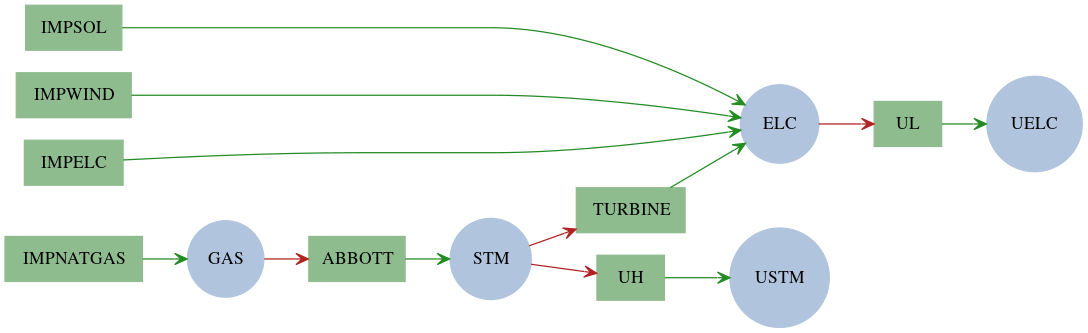
\includegraphics[width=\textwidth]{bau_temoa_uiuc.png}
    \caption{Graph representation of the UIUC embedded grid.}
    \label{fig:uiucgrid}
  \end{figure}
\end{frame}

\begin{frame}
  \frametitle{BAU: Generation}
      \begin{figure}
        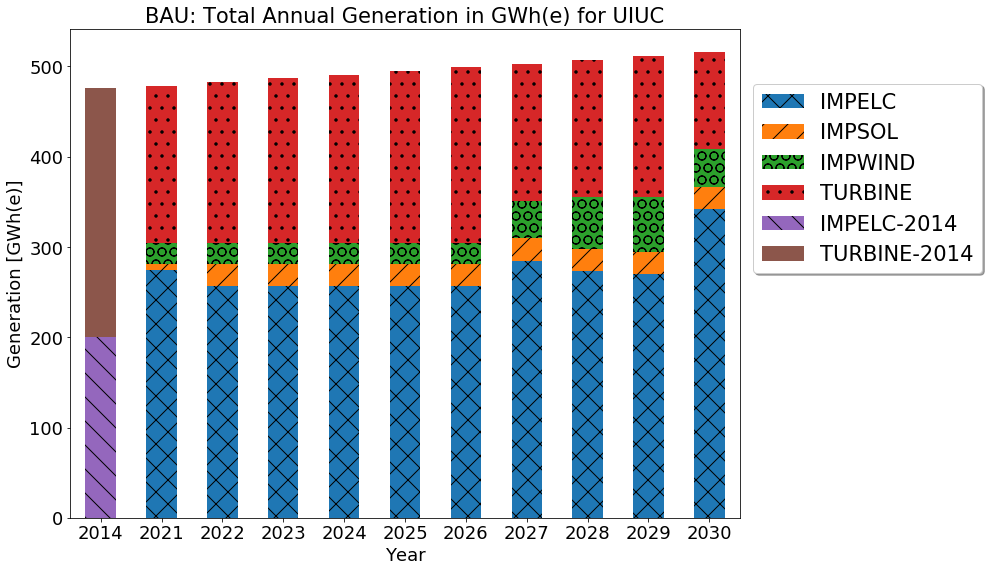
\includegraphics[width=0.8\textwidth]{bau_generation_w2014.png}
        \caption{The change in activity from each energy source from 2020-2030. Assuming 1\% demand growth each year}
        \label{fig:bau_generation}
      \end{figure}

\end{frame}

\begin{frame}
  \frametitle{BAU: Emissions}
  \begin{columns}
    \column[t]{5cm}
      \begin{figure}
        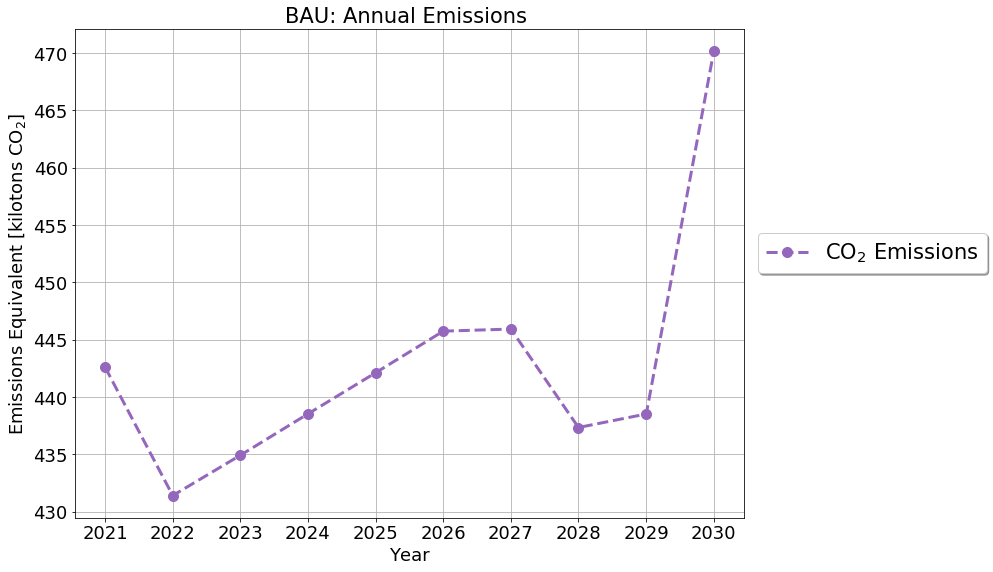
\includegraphics[width=\textwidth]{bau_emissions.png}
        \caption{The change in activity from each energy source from 2020-2030. Assuming 1\% demand growth each year}
        \label{fig:bau_generation}
      \end{figure}
    \column[t]{5cm}
    \begin{figure}
        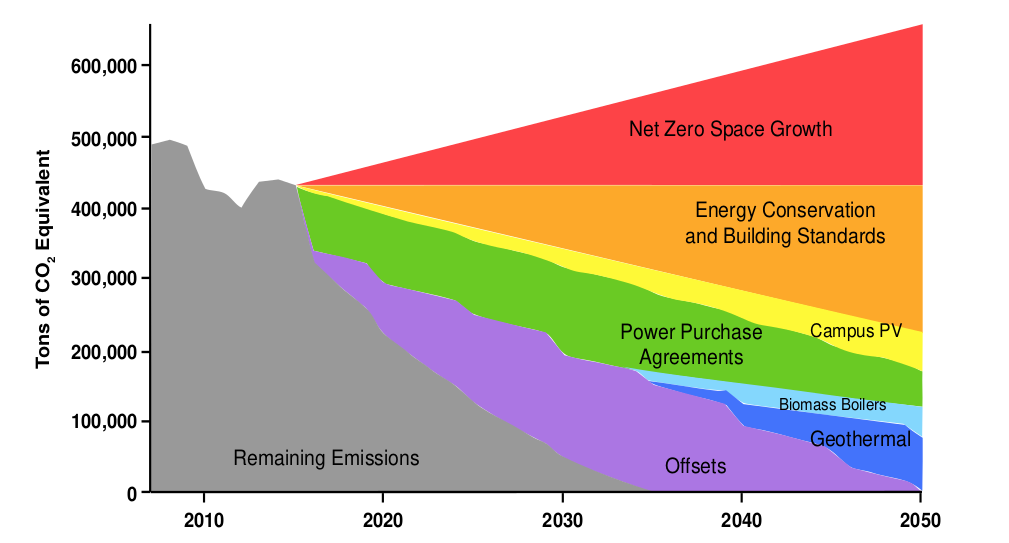
\includegraphics[width=\textwidth]{icap_uiucemissions.png}
        \caption{Predicted growth in emissions from iCAP \cite{isee_illinois_2015}.}
        \label{fig:uiuc_emissions}
      \end{figure}
  \end{columns}
\end{frame}

\subsection{\texttt{Temoa}: Nuclear Scenarios}

\begin{frame}
  \frametitle{Nuclear Scenarios}
  \begin{columns}
    \column[t]{3cm}
    \begin{enumerate}
      \item Scenario 1: Zero Capital Costs
      \item Scenario 2: No Capacity Limit
      \item Scenario 3: Limited to Small Modular Reactor (100MWth)
    \end{enumerate}

    \column[t]{7cm}
    \begin{table}
      \centering
      \caption{Summary of Nuclear Scenarios. Costs from EIA and NEI reports \cite{desai_nuclear_2018}\cite{us_department_of_energy_capital_2016}. Assumes
      thermal efficiency of 33\%.}
      \label{table:scenarios}
      \resizebox{\columnwidth}{!}{
      \begin{tabular}{cccc}
        Scenario & Operation Costs & Capital Costs & Maximum Capacity \\
        & [\$/MWh(th)]& [M\$/MWth] & [MWth] \\
        1 & 8.91 & - & - \\
        2 & 8.91 & 1.982 & - \\
        3 & 8.91 & 1.982 & 100 \\
      \end{tabular}
      }
    \end{table}
  \end{columns}
\end{frame}

\begin{frame}
  \frametitle{Nuclear Scenarios: Grid Model}
  \begin{figure}
    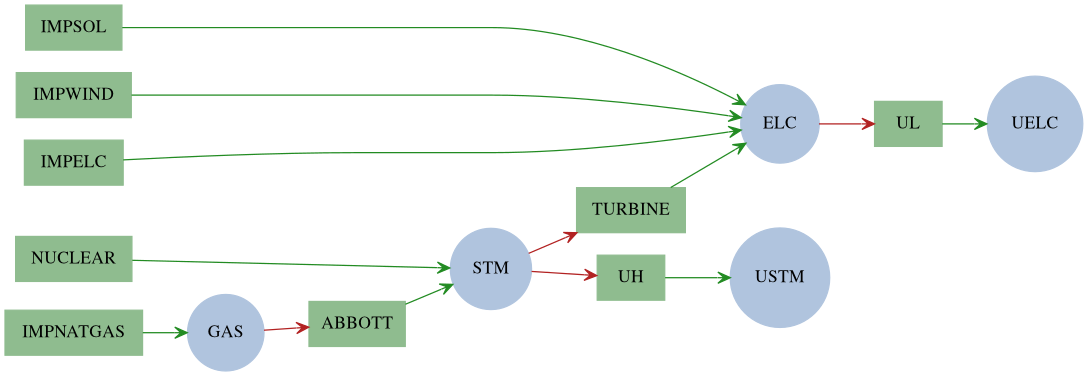
\includegraphics[width=\textwidth]{temoa_uiuc_nuclear.png}
    \caption{Graph representation of the UIUC grid with nuclear reactor.}
    \label{fig:nuclear-uiuc}
  \end{figure}
\end{frame}


\subsection{Scenario 1: Zero Capital Costs}
\begin{frame}
  \frametitle{Scenario 1: Generation}
    \begin{figure}
      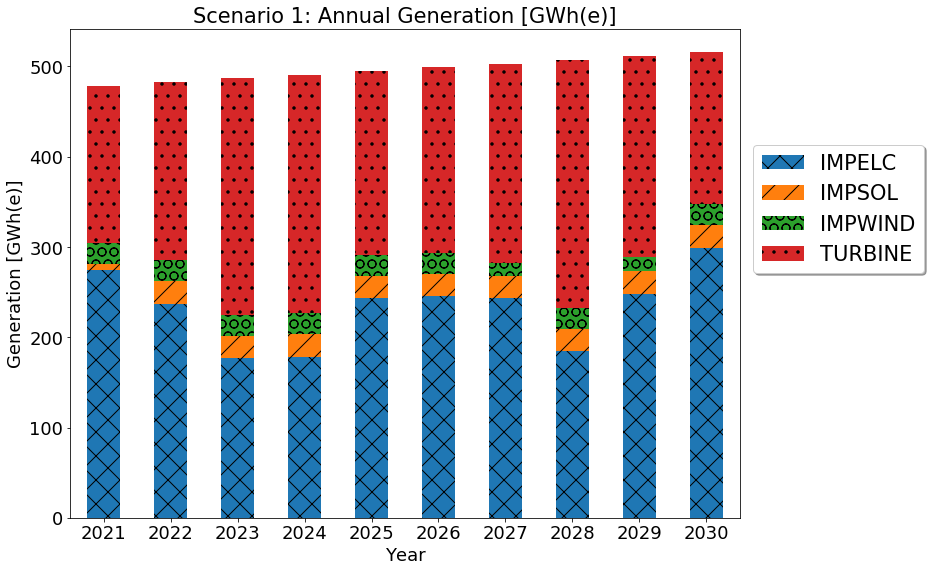
\includegraphics[width=0.9\textwidth]{scenario1_generation.png}
      \caption{The electric generation without a cost constraint on nuclear}
      \label{fig:gen01}
    \end{figure}
\end{frame}
\begin{frame}
  \frametitle{Scenario 1: Emissions}
  \begin{figure}
    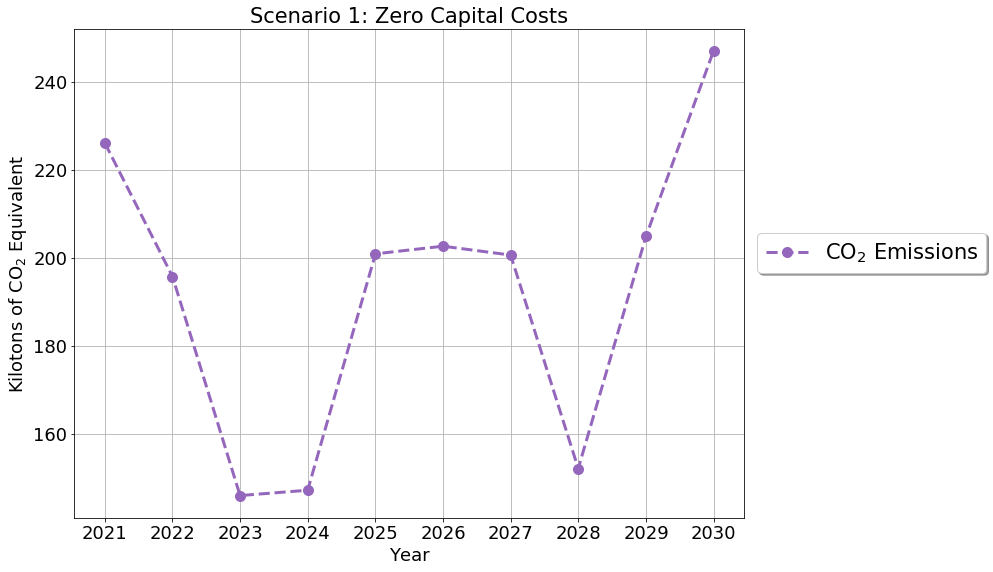
\includegraphics[width=0.9\textwidth]{scenario1_emissions.png}
    \caption{The carbon equivalent emissions without a cost constraint on nuclear}
    \label{fig:emit01}
  \end{figure}
\end{frame}
\subsection{Scenario 2: No Capacity Limit}
\begin{frame}
  \frametitle{Scenario 2: Generation}
  \begin{figure}
    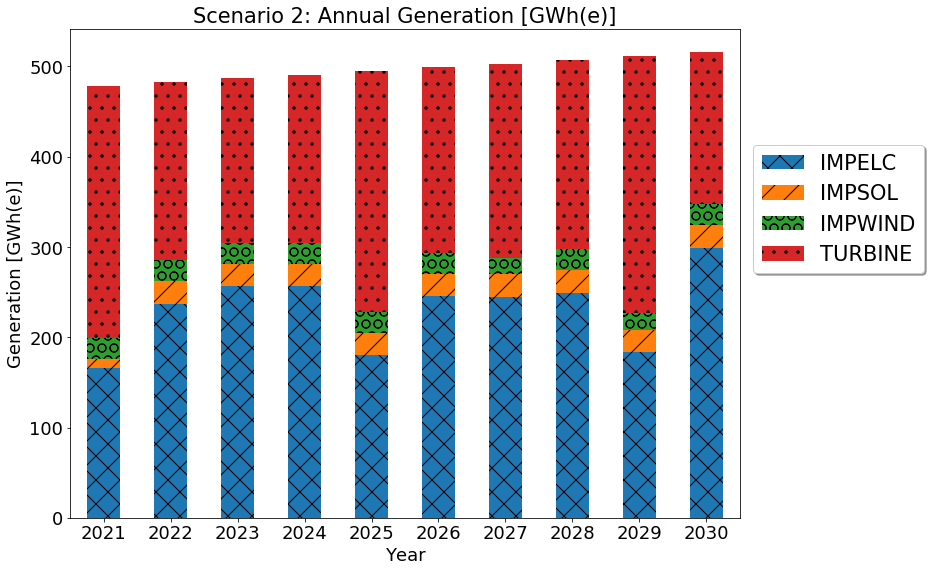
\includegraphics[width=0.9\textwidth]{scenario2_generation.png}
    \caption{The electric generation without a size constraint on nuclear}
    \label{fig:gen02}
  \end{figure}
\end{frame}
\begin{frame}
  \frametitle{Scenario 2: Emissions}
  \begin{figure}
    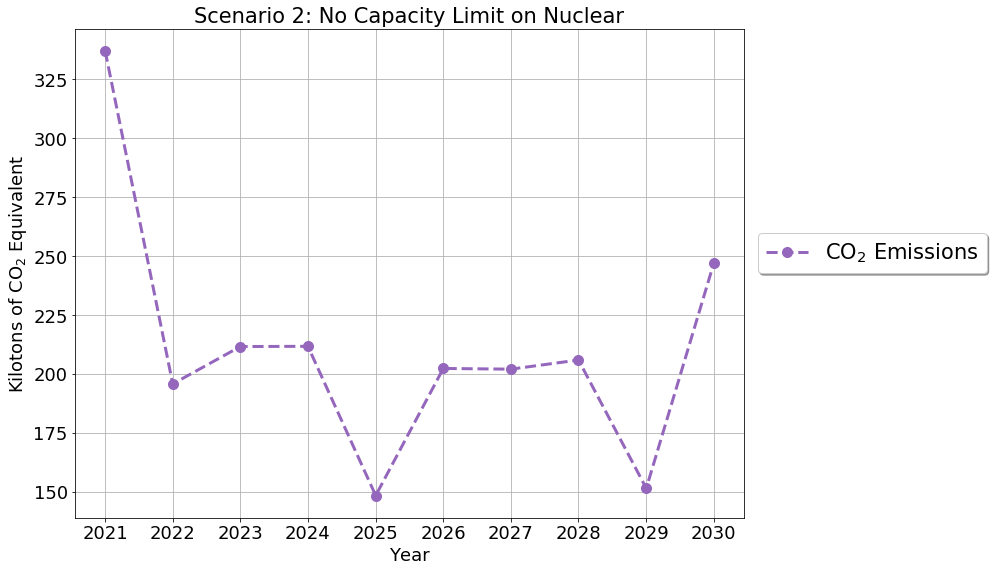
\includegraphics[width=0.9\textwidth]{scenario2_emissions.png}
    \caption{The carbon equivalent emissions without a size constraint on nuclear}
    \label{fig:emit02}
  \end{figure}
\end{frame}
\subsection{Scenario 3: Small Modular Reactor}
\begin{frame}
  \frametitle{Scenario 3: Generation}
  \begin{columns}
    \column[t]{5cm}
    \begin{figure}
      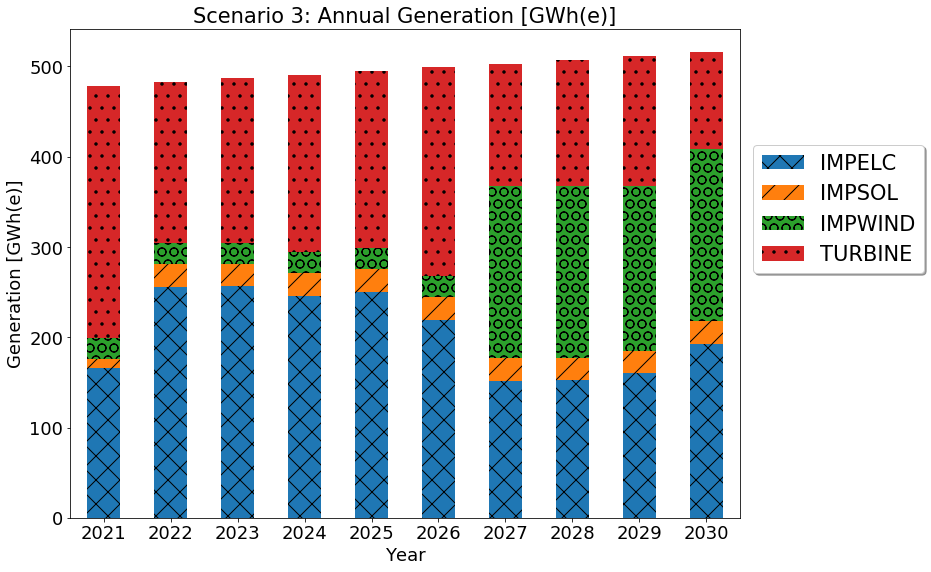
\includegraphics[width=\textwidth]{scenario3_generation_elc.png}
      \caption{The electric generation with constrained nuclear.}
      \label{fig:gen03elc}
    \end{figure}
    \column[t]{5cm}
    \begin{figure}
      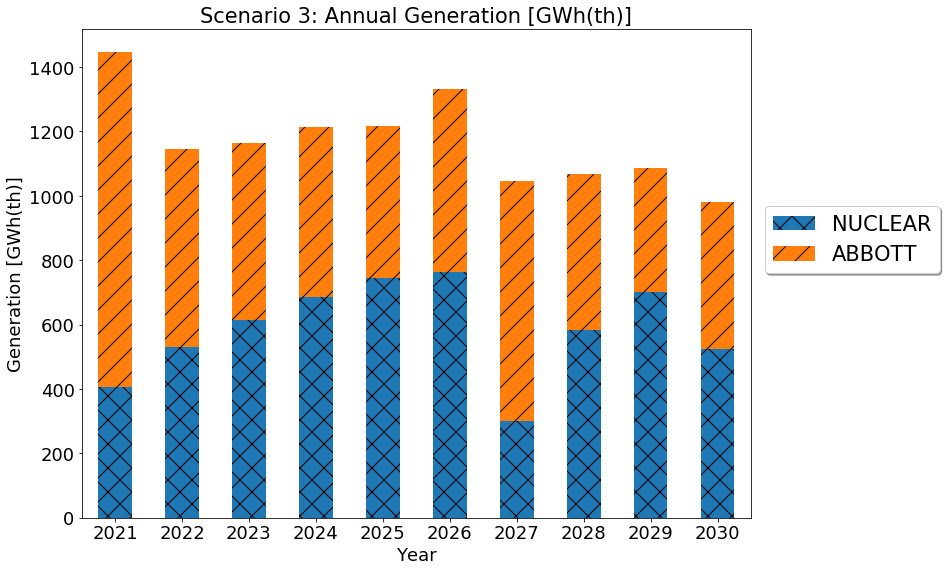
\includegraphics[width=\textwidth]{scenario3_generation_stm.png}
      \caption{The steam generation with constrained nuclear}
      \label{fig:gen02stm}
    \end{figure}
  \end{columns}
\end{frame}
\begin{frame}
  \frametitle{Scenario 3: Emissions}
  \begin{figure}
    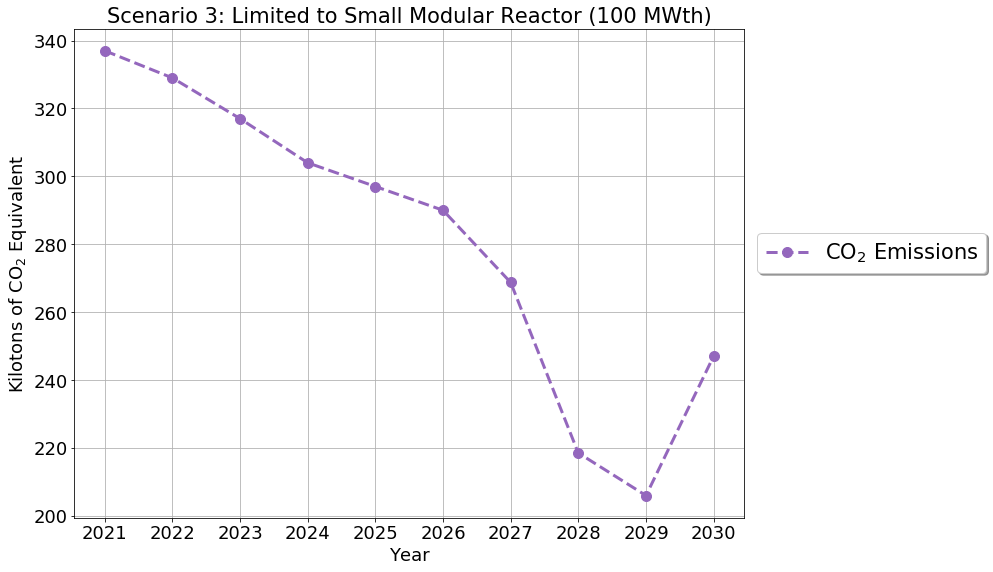
\includegraphics[width=0.9\textwidth]{scenario3_emissions.png}
    \caption{The carbon equivalent emissions without a cost constraint on nuclear}
    \label{fig:emit03}
  \end{figure}
\end{frame}
